\documentclass[12pt, a4paper]{article}

\usepackage[brazilian]{babel}
\usepackage[utf8]{inputenc}
\usepackage[T1]{fontenc}
\usepackage{url}
\usepackage[backend=biber,style=abnt]{biblatex}
\usepackage[autostyle]{csquotes}
\usepackage{authblk}
\usepackage[a4paper, left=3cm, right=2cm, top=3cm, bottom=2cm]{geometry}
\usepackage{setspace}
\usepackage{multirow}
\usepackage{listings}
\usepackage{graphicx}
\usepackage{subcaption}
\usepackage{caption}
\usepackage{wrapfig}

%%% Setup

%lst
\lstdefinestyle{lststyle}{
	belowcaptionskip=1\baselineskip,
	breaklines=true,
	frame=single
}

\renewcommand{\lstlistingname}{Ex}
\lstset{style=lststyle}

%caption
\captionsetup[figure]{font=small}
\captionsetup[lstlisting]{font=small}

%%% Documento
\onehalfspacing
\addbibresource{artigo.bib}

\author{Gabriel Almeida Bueno}
\affil{FATEC Zona Sul}
\title{Tecnologia e Artes, um estudo sobre a tecnologia da informação como meio para compreensão e realização artística}

\begin{document}

\maketitle

\section{Introdução}
% O que é arte? Qual é a sua importância?
A arte é parte indissociável da vivência humana, e a tecnologia é parte indissociável da arte. 
Sendo uma das atividades mais antigas exercidas pelo ser-humano, podemos enxergar características estéticas e manifestações artísticas realizadas pelos vários povos e culturas antigas até a contemporaneidade, seja por meio do artesanato, arquitetura, pintura ou poesia.
O belo sempre é benquisto por qualquer indivíduo que seja, independente do seu meio social ou seus gostos pessoais.
Na Poética, ao definir a arte da poesia, Aristóteles \cite[p.42]{aristotle_poetics} afirma que 

\begin{displayquote}
as coisas que observamos ao natural e nos fazem pena agradam-nos quando as vemos representadas em imagens muito perfeitas.
\end{displayquote}

Cada registro artístico, porém, representa não só algo que é sensivelmente belo, mas constitui uma expressão do indivíduo que o fez, carregando em si
também o espírito da época em que foi realizado, do meio em que o artista estava inserido. 
A arte mostra-se, portanto, de valor inestimável como registro da expressão humana, Da Vinci \cite{davinci_thoughtsonart} diria que:

\begin{displayquote}
Os frutos da pintura podem ser compreendidos por todas as populações do universo pois seus resultados
são sujeitos ao poder da visão [...] não necessitando de intérpretes para as várias línguas.
\end{displayquote}

Identidades religiosas e nacionais também fazem uso da estética, já que historicamente podemos observar que, nas palavras de Hegel \cite{hegel}:

\begin{displayquote}
é nos trabalhos de arte que nações tem depositado as mais ricas intuições e ideias que possuem; e não 
infrequentemente as belas artes fornecem uma chave para a interpretação da sabedoria e religião dos povos.
\end{displayquote}

Já o ato de realizar arte, por outro lado, é estritamente ligado à tecnologia.
As ferramentas criadas pelo homem a fim de subjugar os obstáculos impostos
pelo meio ambiente à sua sobrevivência, foram e sempre serão usadas pelo artista como meio de expressão e para o fazer artístico \cite{gouzouasis}.
A evolução da tecnologia interfere diretamente nas manifestações artísticas, o que podemos notar pela simples observação da arte ao longo da história: das pinturas que passaram das paredes das cavernas para o óleo em tela, até
a fotografia; da música tocada em alaúdes com tripas torcidas até os violões com cordas de nylon, chegando até as guitarras elétricas; 
da gravação e reprodução sonora que partiu do fonógrafo até os computadores e CDs, até o mais recente \emph{streaming}. 
É notório como a tecnologia de uma época pode influenciar nas manifestações artísticas do período. 

Um dos sentidos que o famoso aforismo de McLuhan, "o meio é a mensagem", carrega em si é o de que o 
\emph{meio transforma o seu conteúdo} \cite[p.50]{braga_mcluhan}. 
Um novo meio, fruto de uma inovação tecnológica, impacta na própria mensagem passada na obra artística.
Estamos na era da informação, com capacidade computacional de sobra e uma digitalização crescente do mundo tangível. 
Como a tecnologia contemporânea pode influenciar no estado atual da realização e compreensão artística?

\begin{figure}[ht!]
	\centering
	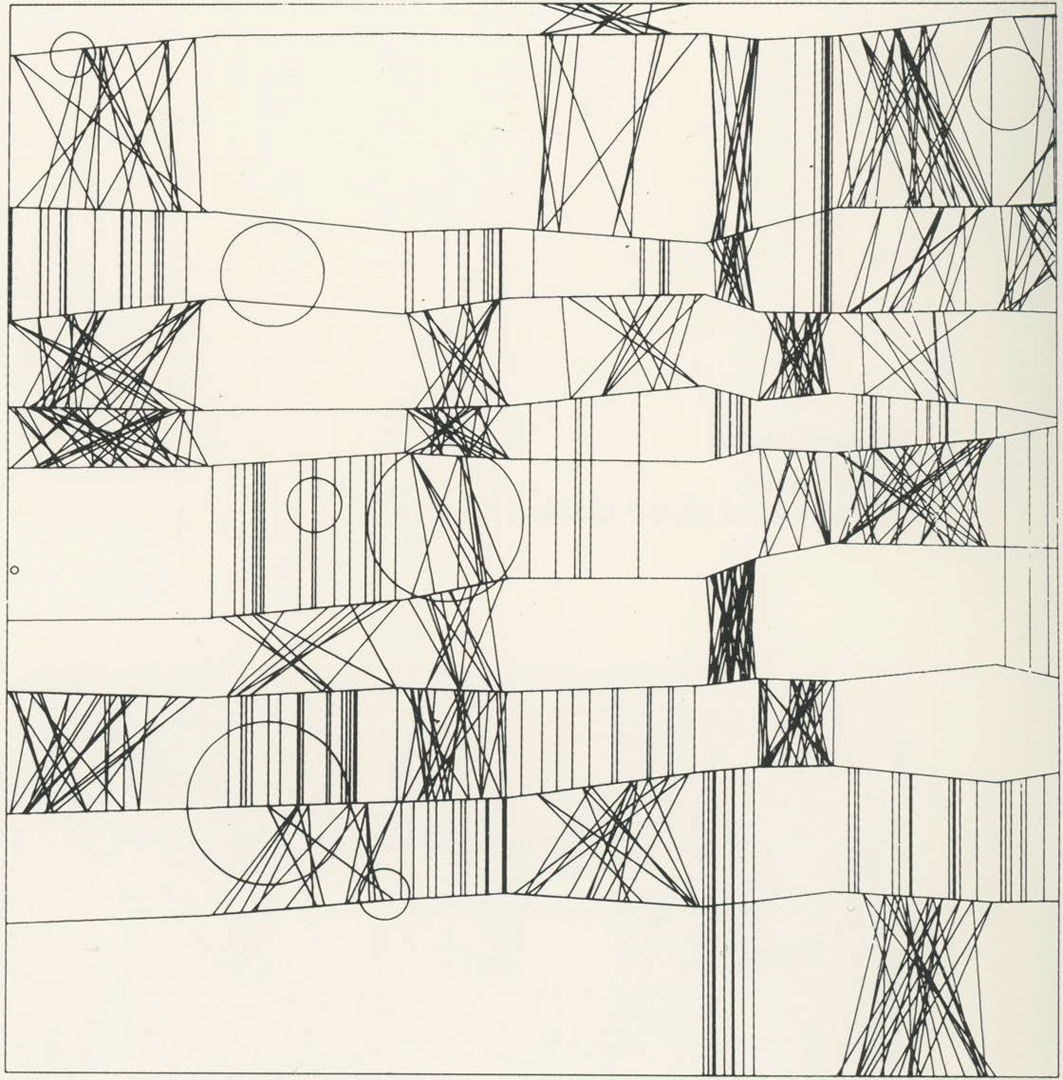
\includegraphics[width=\textwidth, height=7cm, keepaspectratio=true]{fig/hommage_to_paul_klee}
	\caption{
		Obra \emph{Hommage à Paul Klee}, de Frieder Nake, realizada em 1965 \cite{homage_to_paul_klee}.
	}
\end{figure}

\begin{figure}[ht!]
	\centering
	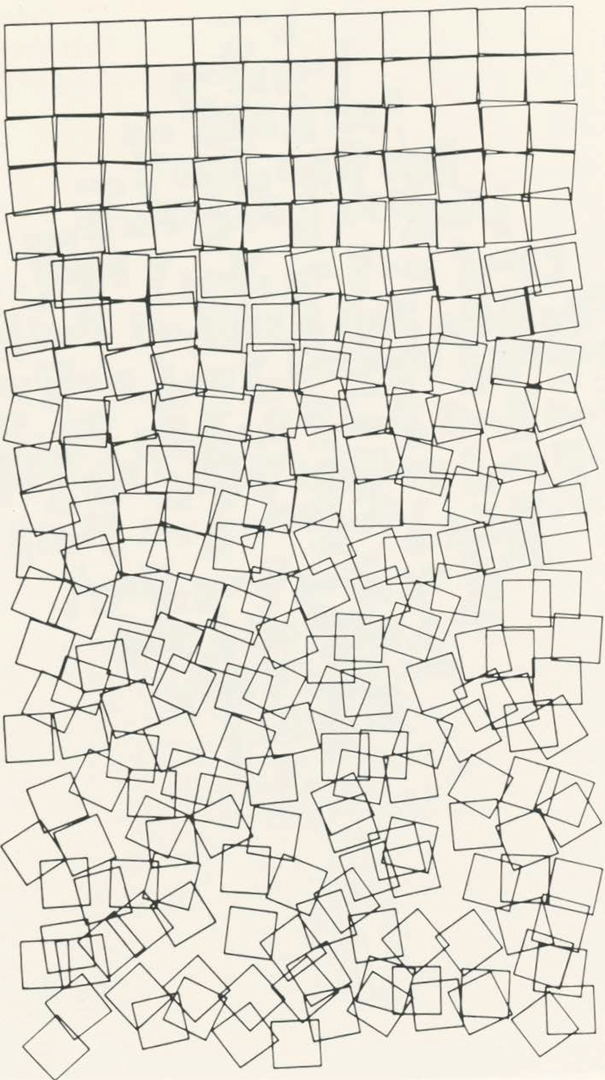
\includegraphics[width=\textwidth, height=7cm, keepaspectratio=true]{fig/gravel_stones}
	\caption{
		\emph{Gravel Stones}, de Georg Nees
		\cite{gravel_stones}.
	}
\end{figure}

Como exemplos do fazer artístico utilizando como meio a tecnologia contemporânea, podemos ressaltar o trabalho
de artistas como Frieder Nake, Georg Nees e Vera Molnar que, em meados dos anos 60, influenciados pela filosofia de Max Bense, vanguardearam 
o movimento da arte algorítmica, conhecido também pelas alcunhas de arte generativa, arte computacional, gráficos generativos, entre outros.
O algoritmo é a principal ferramenta do artista computacional, através do qual a ideia da obra artística é modelada em um programa de computador -- utilizando-se de símbolos, eventos e estados -- que ao ser executado produzirá a obra em si. Neste movimento, o modo convencional do fazer artístico, já conhecido a muito, dá lugar para a ciência e a matemática. 

Vemos que a tecnologia contemporânea já é tão significativa que nos deu novos meios para o fazer artístico, trazendo consigo, além disso, reflexões acerca do próprio ato de fazer arte, já que a ideia de arte feita "pelo computador" não é aceita de bom grado pelo crítico
mais conservador.
Ora, não há de se negar que o matemático, cientista ou engenheiro mais romântico, apesar de não necessariamente chamar de arte, indubitavelmente enxerga alguma forma de beleza na atividade que exerce e nos frutos de seu trabalho. 
Na sua apologia, Hardy \cite{hardy_apology} escreve:

\begin{displayquote}
Um matemático, como um pintor ou poeta, é um criador de padrões. Se os padrões daquele são mais permanentes do que os destes, é porque eles são feitos com ideias.
\end{displayquote}

Ao lamentar a forma como a matemática é ensinada para as crianças em nível escolar (sua lamentação poderia muito bem ser transposta para o próprio ensino de arte), Lockhart \cite{lockhart_lament} expressa que:

\begin{displayquote}
Nenhuma sociedade jamais reduziria uma forma tão bela e significativa de arte para algo tão insignificante e trivial. Nenhuma cultura poderia ser tão cruel com suas crianças a ponto de privá-las de um meio tão satisfatório e natural de expressão humana.
\end{displayquote}

A sociedade cada vez mais vê-se de todo tomada pela digitalização. Se o homem se torna digital, sua expressão em forma de 
manifestação artística se tornará, também, digital. Como isso impactará no ensino vigente da arte?
Há a necessidade de se apresentar ao aluno a tecnologia contemporânea como forma de realização e estudo da arte.
Os três pilares da abordagem triangular de Ana Mae Barbosa -- o conhecimento da história, a apreciação da arte, e o próprio fazer artístico --
deveriam ser extendidos para abranger também a arte produzida pelos meios contemporâneos ao aluno.
É evidente que a tecnologia não é uma panaceia para resolver todos os problemas da educação artística, porém, a tecnologia atual, já que é parte
inseparável do indivíduo, deve, de alguma forma e em algum momento, nem que breve, ser abordada a fim de contextualizá-lo na sociedade em que vive.

Tendo em vista esta natureza inerentemente tecnológica da arte, em contraponto com a aparente falta de diálogo entre o meio artístico e o campo
mais recente do desenvolvimento tecnológico -- algo que pode ser observado empiricamente em certos meios -- este trabalho apresenta-se com o objetivo
de relacionar uma das tecnologias que mais vem recebendo atenção dos pesquisadores e engenheiros -- a das inteligências artificiais, mais especificamente,
o das \emph{redes neurais} -- com o meio da arte. 
Uma breve revisão das inteligências artificiais e das redes neurais será feita a fim de, para contextualizar o assunto, criar uma base 
histórica e teórica do assunto, além de citar outros trabalhos realizados na área que possuem alguma relação com a arte.
Como estudo de caso e exemplo de aplicação prática, um sistema de rede neural capaz de tentar categorizar o estilo artístico
de uma pintura foi criado. Este sistema mostra uma possível forma de integração de uma rede neural com o meio artístico, 
abrindo ainda mais possibilidades para a criação e evolução de sistemas de informação na arte, seja como ferramenta para auxílio a educação ou para a própria realização artística. 
Para tentar detectar o interesse popular da abordagem de tecnologia no ensino artístico, como uma forma de testar a hipótese de
que é necessário pelo menos uma abordagem eventual da tecnologia recente na arte, uma pesquisa foi conduzida com aproximadamente 70 pessoas. Seus resultados
também serão exibidos neste trabalho.

\section{Referencial teórico}
\subsection{Uma breve história da IA e das Redes Neurais}
\begin{displayquote}
Portanto o bem é instrumento para a existência, uma propriedade é uma multitude de instrumentos; então o escravo é um instrumento animado,
mas qualquer um capaz de agir por si só é mais valioso do que qualquer outro instrumento; pois se cada instrumento, em um comando,
ou por uma pré-concepção da vontade de seu mestre, pudesse realizar seu trabalho (como diz a história sobre as estátuas de Dédalo; ou o que
o poeta nos canta dos tripés de Hefesto, que à própria vontade se moviam ao conclave dos Deuses), a lançadeira então teceria, e a lira
tocaria a si mesma; nem o arquiteto desejaria servos, nem o mestre escravos. \cite{aristotle_politics}
\end{displayquote}

A construção de máquinas autônomas, capazes de agir à semelhança de seus criadores, não é uma ideia recente, mas sim remonta à tempos antigos. 
O exigente escultor Pigmalião e sua Galatéia; as estátuas de Dédalo; Pandora, criação de Hefesto e punição Jupiteriana, 
são exemplos de mitos que tem em si a ideia da criação de uma vida artificial. 
O surgimento das ciências da computação e das máquinas programáveis fizeram ressurgir a chama destes mitos, 
fazendo-nos nos questionar se um dia estas máquinas se tornariam inteligentes. \emph{Inteligência}, porém, por si só, é um conceito ambíguo.
A discussão sobre \emph{máquinas inteligentes}, por consequência, depende de uma definição precisa de inteligência.

Ao propor a questão "podem máquinas pensar?", Alan Turing apresenta uma abordagem comportamental -- hoje conhecida como \emph{Teste de Turing} --
para determinar se uma máquina é ou não inteligente. Turing propõe que um juíz, isolado dos demais participantes,
tenha uma conversa, em linguagem natural, com um humano e com uma máquina que simula um comportamento humano.
Se no fim da conversa o juíz não for capaz de distinguir a máquina do humano, pode-se afirmar que a máquina é \emph{inteligente}
\cite{turing}. Descartes, em seu Discurso do Método, discorre sobre um assunto semelhante ao de Turing em seu artigo, ao elaborar como se diferenciam
uma máquina de um humano.

\begin{displayquote}
E detivera-me particularmente neste ponto, para mostrar que, se houvesse máquinas assim, que tivessem os órgãos e a figura de um macaco,
ou qualquer outro animal sem razão, não disporíamos de nenhum meio para reconhecer que elas não seriam em tudo da mesma natureza que esses animais;
ao passo que, se houvesse outras que apresentassem semelhança com os nossos corpos e imitassem tanto nossas ações quanto moralmente fosse possível,
teríamos sempre dois meios muito seguros para reconhecer que nem por isso seriam verdadeiros homens. Desses, o primeiro é que nunca poderiam usar palavras,
nem outros sinais, compondo-os, como fazemos para declarar aos outros os nossos pensamentos. Pois pode-se muito bem conceber que uma máquina seja feita de tal modo que profira palavras, e até que profira algumas a propósito das ações corporais que causem qualquer mudança em seus órgãos: por exemplo,
se a tocam num ponto, que pergunte o que se lhe quer dizer; se em outro, que grite que lhe fazem mal, e coisas semelhantes;
mas não que ela as arranje diversamente, para responder ao sentido de tudo quanto se disser na sua presença, assim como podem fazer os homens mais embrutecidos. E o segundo é que, embora fizessem muitas coisas tão bem, ou talvez melhor do que qualquer de nós, falhariam infalivelmente em algumas outras,
pelas quais se descobriria que não agem pelo conhecimento, mas somente pela disposição de seus órgãos. \cite{descartes}
\end{displayquote}

Este parágrafo que Descartes escreve em 1637 serve muito bem para definir o estado atual da computação e a motivação da inteligência artificial.
Com os modelos computacionais que temos atualmente, 
é simples a resolução de problemas que se mostram complexos para um humano, 
desde que o dito problema seja quantificável e reduzível, possível de ser descrito formalmente.
A realização de tarefas como reconhecer falas, sentimentos, faces ou expressões, que constituem o que é ser humano e é feito de forma
automática e intuitiva por nós, se mostra extremamente difícil de ser descrito formalmente em um modelo computacional.
O campo da inteligência artificial serve, portanto, para tentar criar sistemas que realizam estas tarefas humanamente simples porém 
computacionalmente complexas, da forma mais semelhante à humana possível.

\subsubsection{Dartmouth e o início da IA}

\begin{figure}[ht!]
	\centering
	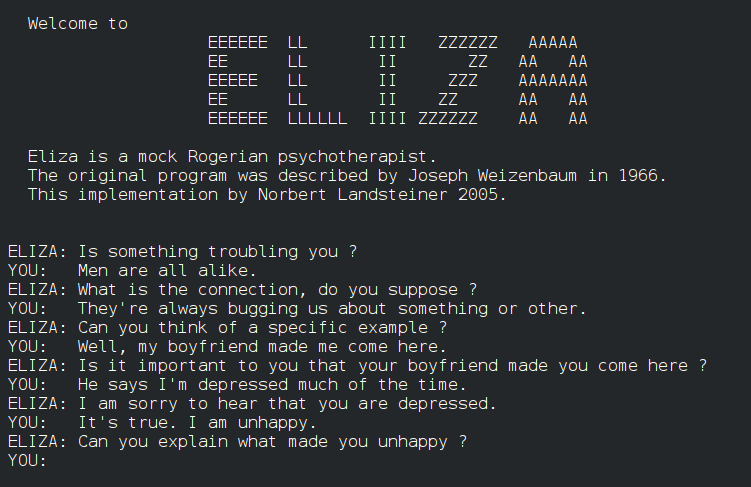
\includegraphics[width=\textwidth, height=7cm, keepaspectratio=true]{fig/eliza}
	\caption{
		Uma conversa com \emph{ELIZA}. Imagem em domínio público retirada da \emph{Wikipedia}
		\cite{wikipedia_eliza}.
	}
\end{figure}

Apesar da IA, como ferramenta computacional, parecer ser um assunto recente, 
pertencente à vanguarda da corrida tecnológica atraindo a atenção de estudantes e empresários, sua pesquisa
remonta pelo menos aos anos 50.
A conferência de Dartmouth, em 1956, foi um dos primeiros movimentos que impulsionaram o início das 
pesquisas em inteligência artificial. \cite{dartmouth}.
As redes neurais e o uso de linguagem natural pelo computador -- assuntos que permanecem ainda atuais --, entre outros tópicos de discussão,
foram alvo de trabalho pelos pesquisadores que participaram da conferência. 
Durante as primeiras décadas de pesquisa foram concebidos trabalhos importantíssimos para suportar o cenário da IA que temos atualmente.
\emph{ELIZA} \footnote{http://psych.fullerton.edu/mbirnbaum/psych101/eliza.htm}, 
uma simulação de um psicoterapeuta rogeriano, desenvolvida por Joseph Weizembaum no MIT Artifical Intelligence Laboratory de 1964 até 1966,
foi o primeiro chatbot desenvolvido na história, com o objetivo de demonstrar como a comunicação máquina-homem é superfifical \cite{wiezembaum}.
Outro trabalho pioneiro é o de Daniel G. Bobrow, que na sua tese de PhD em 1964 desenvolve o STUDENT, uma IA escrita em LISP para solucionar problemas
de álgebra \cite{student}.

\subsubsection{IA Simbólica e Aprendizado de Máquina}
\begin{wrapfigure}{r}{0.30\textwidth}
	\begin{center}
		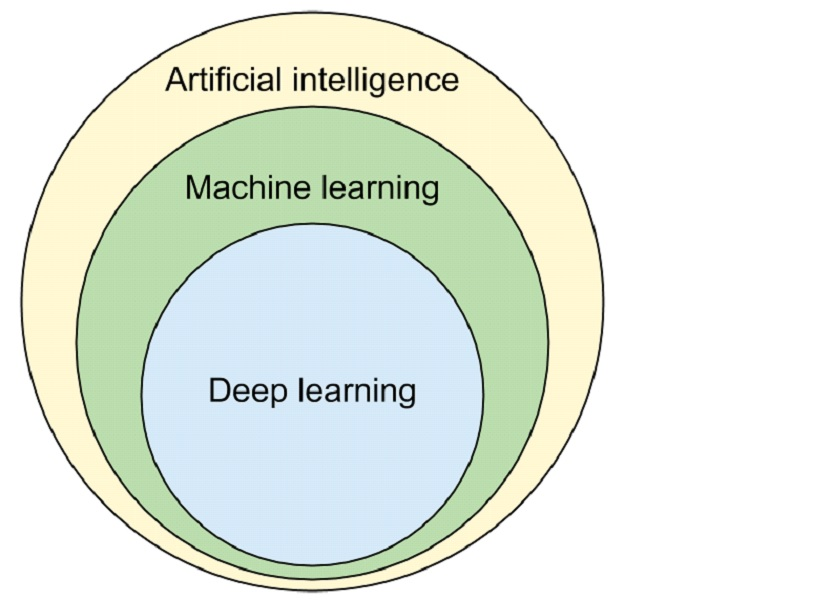
\includegraphics[width=0.28\textwidth]{fig/ml_venn}
	\end{center}
	\caption{
		Deep Learning é um subcampo do Machine Learning, que por sua vez é um subcampo da Inteligência Artificial.
		Imagem do Wikipedia
		\cite{wikipedia_ml}.
	}
\end{wrapfigure}
O cerne principal da escrita de algoritmos -- em qualquer problema de computação, não somente na IA --, 
é a \emph{representação de dados} utilizada para resolver o determinado problema. A \emph{IA simbólica},
tipo de IA que mais ocupou o tempo e os esforços dos pesquisadores da década de 80, tenta representar o conhecimento
sobre o mundo por \emph{fatos} e \emph{símbolos} atômicos através dos quais se pode realizar deduções e inferências. 
O Cyc, um projeto cuja ambição era o de criar uma
base de dados com uma quantidade considerável do conhecimento comum da humanidade, através do qual
novo conhecimento poderia ser deduzido através do seu motor de inferência \cite{cyc}, serviria de exemplo para outros sistemas
que utilizariam a mesma abordagem de IA. A linguagem Prolog \footnote{https://www.swi-prolog.org/}, 
desenvolvida por Alain Colmerauer conjuntamente com Philippe Roussel em Marselha, 1972, 
foi uma das primeiras linguagens de programação com paradigma lógico, tendo suas raízes na teoria de lógica de primeira ordem.
Nesta linguagem, os problemas são modelados por \emph{átomos} e \emph{regras} que estabelecem relações entre os átomos.
O Prolog viu sua aplicação em trabalhos de IA na criação de sistemas especialistas, processamento de linguagem natural, entre outros. 
Apesar dos esforços, a IA simbólica não demonstrou muito sucesso. Suas dificuldades e empecilhos sugerem que os sistemas de inteligência
artifical, para se mostrarem eficazes, deveriam ser capazes de por si só adquirir o próprio conhecimento necessário
para a resolução de um problema \cite{Goodfellow-et-al-2016}.

\bigskip
\begin{lstlisting}[caption={Exemplo do uso da linguagem Prolog para modelar a famosa proposição da mortalidade de Sócrates.}, captionpos=b]
homem(socrates).
mortal(X) :- homem(X).
\end{lstlisting}

Como resposta a este problema surgem as técnicas de \emph{aprendizado de máquina}. Estas técnicas e algoritmos
baseiam-se na capacidade de, a partir de massas não estruturadas de dados, extrair padrões que
possibilitem a solução ou previsão de um problema  \cite{Goodfellow-et-al-2016}.
Regressão linear, regressão logística, classificadores Bayes ingênuos, 
kNN e k-means são exemplos de técnicas de aprendizado de máquina.
Nota-se que boa parte do ferramentário deste campo da inteligência artificial utiliza-se de modelos estatíscos para extrair informações
dos dados não estruturados. Algumas destas técnicas de aprendizado de máquina, porém, não lidam com o problema da \emph{representação}
dos dados, sendo esta estaticamente definida de acordo com o problema que está sendo atacado e a sua natureza. O algoritmo simplesmente mapeia uma representação de dados para uma saída que representa, por exemplo, uma probabilidade.
Como já elaborado anteriormente, algumas das tarefas simples para a realização por um humano são complexos de serem modelados computacionalmente;
portanto, para a criação de sistemas inteligentes que realizam estas tarefas não há somente o problema da coleta de informações e conhecimento,
mas também o da própria \emph{representação}. 
As técnicas de aprendizado de máquina podem ser utilizadas não só para, a partir de uma representação pré-definida, produzir uma resposta ao problema, mas também para automaticamente descobrir, por si só, a representação ideal.

Ao criar uma representação que modela um problema do mundo real para um algoritmo de aprendizado de máquina -- ou mesmo para modelar o próprio algoritmo de aprendizado da representação -- há de se detectar e separar os \emph{fatores de influência} deste problema. Estes fatores não necessariamente são discretos, mas são quaisquer características que determinam a saída correta para um conjunto de dados em uma determinada representação. Em um nível mais alto, os fatores de influência são, por exemplo, as características que determinam a essência de algo, o que este algo é -- uma pintura, por exemplo, apresenta cores e formas que fazem com que o observador saiba de imediato que objeto foi ali representado. Estes fatores de influência muitas vezes são constituídos de ideias cujo significado total depende de interpretações extritamente ligadas à linguagem humana, não sendo possível a sua tradução fiel em uma linguagem simbólica formal. O \emph{Deep Learning} surge como técnica de aprendizagem de representação que baseia-se em níveis de representações encadeadas sucessivamente que transformam uma entrada na sua respectiva saída \cite{Goodfellow-et-al-2016}. 
No artigo que propõe a conferência de Dartmouth já se apresenta a ideia central das redes neurais, "como um conjunto de nêurons hipotéticos podem ser arranjados para que possam formar conceitos?" foi a questão apresentada \cite{dartmouth}.

\subsection{Redes Perceptron}
\subsection{Redes Neurais Convolucionais (CNNs)}
\subsection{Redes Neurais Adversariais (GANs)}
\subsection{Transferência de Aprendizado}
\subsection{Frameworks atuais para o treinamento de Redes Neurais}

% \nocite{*}
\printbibliography

\end{document}